\chapter{Световые конусы, геодезические и горизонт Шварцшильда}

Проблема горизонта начинается с различия, уже присутствующего в специальной теории относительности. Два близких события могут быть разделены времениподобным, пространственноподобным или светоподобным образом. Кривизна не отменяет этой классификации. Она делает световой конус локальным объектом, различным в каждом событии, и делает саму метрику динамической. Как только метрика известна, движение свободно падающей частицы следует из того же принципа собственного времени, который описывает свободную релятивистскую частицу в плоском пространстве-времени.

Мы воспользуемся этим принципом дважды. Сначала он должен воспроизвести ньютоновское движение в слабом поле. Затем он будет применён к метрике Шварцшильда, где смысл времени, радиального расстояния и скорости неожиданно становится тонким.

\section{Времениподобные, пространственноподобные и светоподобные интервалы}

В плоском пространстве-времени при \(c=1\) элемент собственного времени имеет вид
\begin{equation}
d\tau^2=dt^2-dx^2-dy^2-dz^2.
\label{eq:l5-minkowski-proper-time}
\end{equation}
Явно восстановить \(c\) полезно всякий раз, когда уместно нерелятивистское приближение:
\begin{equation}
d\tau^2
=dt^2-\frac{dx^2+dy^2+dz^2}{c^2}.
\label{eq:l5-minkowski-c}
\end{equation}
Обозначение \(d\tau^2\) не гарантирует, что правая часть положительна. Ее знак классифицирует смещение:
\begin{align}
d\tau^2>0
&\quad\Longleftrightarrow\quad \text{time-like},\\
d\tau^2=0
&\quad\Longleftrightarrow\quad \text{light-like},\\
d\tau^2<0
&\quad\Longleftrightarrow\quad \text{space-like}.
\end{align}
Для пространственноподобного смещения удобно определить положительное собственное расстояние
\begin{equation}
ds^2=-d\tau^2
=dx^2+dy^2+dz^2-dt^2
\qquad(c=1).
\label{eq:l5-proper-distance}
\end{equation}

Световой конус упорядочивает эти три возможности. Из светоподобных направлений состоит его поверхность, а не заполненная внутренняя область. Времениподобные направления лежат внутри конуса, а пространственноподобные — вне его. Верхняя и нижняя половины представляют соответственно будущий и прошлый световые конусы.

\begin{figure}[htbp]
\centering
\includegraphics[width=0.82\textwidth]{lecture_05_figure_02.png}
\caption{Собственное время, собственное расстояние и причинный конус, собранные на доске. Световые лучи лежат на самом конусе; внутренняя область времениподобна, а внешняя — пространственноподобна.}
\lectureframe{00:05:44}
\end{figure}

\begin{figure}[htbp]
\centering
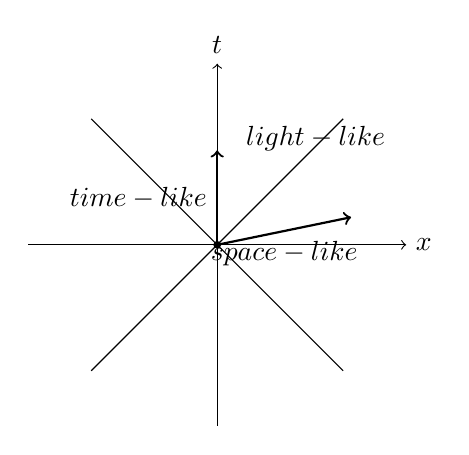
\begin{tikzpicture}[scale=1.0]
\draw[->] (0,-2.3) -- (0,2.3) node[above] {\(t\)};
\draw[->] (-2.4,0) -- (2.4,0) node[right] {\(x\)};
\draw (-1.6,1.6) -- (0,0) -- (1.6,1.6);
\draw (-1.6,-1.6) -- (0,0) -- (1.6,-1.6);
\fill (0,0) circle (1.4pt);
\draw[->,thick] (0,0) -- (0,1.2)
  node[midway,left] {\(\text{time-like}\)};
\draw[->,thick] (0,0) -- (1.7,0.35)
  node[midway,below] {\(\text{space-like}\)};
\node at (1.25,1.35) {\(\text{light-like}\)};
\end{tikzpicture}
\caption{Причинная классификация на двумерном сечении пространства-времени.}
\end{figure}

Эти интервалы определяются операционально. Собственное время — это то, что показывают часы, которые несут вдоль времениподобной мировой линии. Собственное расстояние — это то, что измеряет подходящий набор метровых стержней между пространственноподобно разделёнными событиями. Это не просто названия знаков в квадратичной форме.

\section{Лоренцева сигнатура и конус в каждом событии}

При соглашении о сигнатуре с тремя плюсами плоская метрика имеет компоненты
\begin{equation}
\eta_{\mu\nu}=\operatorname{diag}(-1,1,1,1),
\label{eq:l5-eta}
\end{equation}
и
\begin{equation}
d\tau^2=-\eta_{\mu\nu}\,dx^\mu dx^\nu.
\label{eq:l5-proper-time-eta}
\end{equation}
Выписанная матрица — это выражение тензора второго ранга в одном особенно простом базисе. Ее инвариантная характеристика — сигнатура: одно отрицательное и три положительных направления,
\begin{equation}
\operatorname{signature}(\eta)=(-,+,+,+).
\label{eq:l5-lorentz-signature}
\end{equation}
Метрика с двумя отрицательными знаками имела бы два временных направления. Такие сигнатуры можно изучать математически, но они не описывают пространство-время, предполагаемое здесь.

В искривлённом пространстве-времени компоненты меняются:
\begin{equation}
g_{\mu\nu}=g_{\mu\nu}(x).
\label{eq:l5-position-metric}
\end{equation}
В каждом событии метрика всё равно должна иметь лоренцеву сигнатуру. Следовательно, у каждого события есть свои времениподобные направления, светоподобная граница и пространственноподобные направления. На координатном рисунке конусы могут от точки к точке выглядеть наклонёнными или сжатыми, но причинная классификация сохраняется.

\begin{figure}[htbp]
\centering
\includegraphics[width=0.86\textwidth]{lecture_05_figure_03.png}
\caption{Метрика \(g_{\mu\nu}(x)\), зависящая от положения, причинные обозначения и наброски локальных световых конусов.}
\lectureframe{00:09:41}
\end{figure}

\begin{figure}[htbp]
\centering
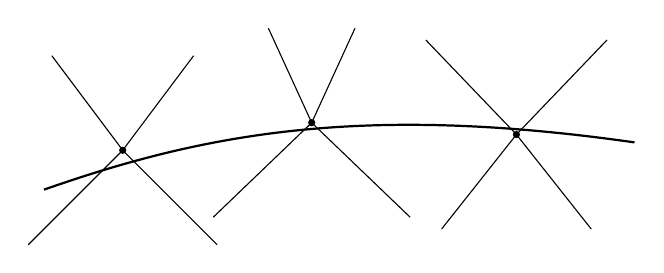
\begin{tikzpicture}[scale=1.0]
\draw[thick] (-4,-0.5) .. controls (-2,0.2) and (0,0.6) .. (3.5,0.1);
\foreach \x/\y/\a/\b in {-3/0/0.9/1.2, -0.6/0.35/0.55/1.25,
                          2.0/0.2/1.15/0.95} {
  \fill (\x,\y) circle (1.3pt);
  \draw (\x,\y) -- ++(-\a,1.2);
  \draw (\x,\y) -- ++(\a,1.2);
  \draw (\x,\y) -- ++(-\b,-1.2);
  \draw (\x,\y) -- ++(\b,-1.2);
}
\end{tikzpicture}
\caption{Соседние локальные конусы. Их координатная форма может меняться без изменения того, какие векторы являются времениподобными, светоподобными или пространственноподобными.}
\end{figure}

\begin{classroomqa}
\audiencequestion{Выделяет ли единственное отрицательное собственное значение одно-единственное временное направление?}
\lecturerresponse{Базис, диагонализующий выписанную матрицу, имеет одно отрицательное базисное направление, но это не выделяет ни предпочтительного наблюдателя, ни одно-единственное физически выделенное направление. Преобразования Лоренца смешивают временную координату с пространственными, и каждый вектор внутри конуса является времениподобным. Инвариантным объектом является конус вместе с сигнатурой с одним минусом и тремя плюсами, а не какой-то один выделенный времениподобный вектор.
\lecturetimestamp{00:12:17--00:17:24}}
\end{classroomqa}

\begin{classroomqa}
\audiencequestion{Почему два рисунка локального конуса могут иметь разную форму?}
\lecturerresponse{Рисунок могут менять координаты. Например, замена \(x\) на координату с другим масштабом меняет численный наклон, приписываемый световому лучу, и тем самым заставляет конус казаться уже или шире. Более общие координаты могут его наклонять. При этом изображаются то же самое событие и те же причинные отношения. В искривлённом пространстве-времени конусы в разных событиях к тому же принадлежат разным касательным пространствам, поэтому для их сравнения требуются метрика и правило переноса.
\lecturetimestamp{00:13:37--00:15:59}}
\end{classroomqa}

\section{Геодезические как вариационная задача}

Свободно движущаяся частица следует по геодезической пространства-времени. В дифференциальной форме, с использованием аффинного параметра \(\lambda\),
\begin{equation}
\frac{d^2x^\mu}{d\lambda^2}
+\Gamma^\mu{}_{\rho\sigma}
\frac{dx^\rho}{d\lambda}
\frac{dx^\sigma}{d\lambda}=0.
\label{eq:l5-geodesic}
\end{equation}
Связность задаёт, как касательный вектор должен оставаться параллельным самому себе при движении частицы.

Существует и вторая формулировка, с которой вычисления часто проще. В римановом пространстве с метрикой \(g_{mn}\) длина кривой равна
\begin{equation}
s=\int ds
=\int\sqrt{g_{mn}\,dx^m dx^n}.
\label{eq:l5-spatial-length}
\end{equation}
Геодезическая делает эту длину стационарной при малых вариациях пути с фиксированными концами. Интеграл есть просто сумма бесконечно малых длин вдоль кривой, а его уравнение Эйлера--Лагранжа — это дифференциальное уравнение второго порядка, аналогичное по форме закону силы.

Для времениподобной мировой линии пространственная длина заменяется собственным временем:
\begin{equation}
\tau
=\int\sqrt{-g_{\mu\nu}\,dx^\mu dx^\nu}.
\label{eq:l5-proper-time-functional}
\end{equation}
Времениподобная геодезическая делает \(\tau\) стационарным и, среди близких свободно падающих путей до появления сопряжённых точек, локально максимальным. Умножение на \(-m\) даёт действие частицы
\begin{equation}
A=-m\tau
=-m\int\sqrt{-g_{\mu\nu}\,dx^\mu dx^\nu}.
\label{eq:l5-particle-action}
\end{equation}
Тем самым тот же путь локально минимизирует \(A=-m\tau\). Различение между стационарностью собственного времени и знаком выбранного действия снимает кажущуюся двусмысленность между минимумом и максимумом.

\section{От собственного времени к обычному лагранжиану}

Действие из \eqref{eq:l5-particle-action} геометрично, но его можно привести к привычной форме, используемой в механике. Параметризуем мировую линию координатой \(t\), разделим каждый дифференциал на \(dt\) и вынесем оставшийся множитель \(dt\) из-под квадратного корня:
\begin{align}
A
&=-m\int\sqrt{-g_{\mu\nu}(x)\,dx^\mu dx^\nu}\\
&=-m\int
\sqrt{-g_{\mu\nu}(x)
\frac{dx^\mu}{dt}\frac{dx^\nu}{dt}}\,dt.
\label{eq:l5-action-t}
\end{align}
Для временной компоненты \(dt/dt=1\); пространственные компоненты — это обычные координатные скорости. Поэтому можно записать
\begin{equation}
\begin{aligned}
A&=\int L\,dt,\\
L&=-m\sqrt{-g_{\mu\nu}(x)\dot x^\mu\dot x^\nu},\\
\dot x^\mu&=\frac{dx^\mu}{dt}.
\end{aligned}
\label{eq:l5-relativistic-lagrangian}
\end{equation}

\begin{figure}[htbp]
\centering
\includegraphics[width=0.88\textwidth]{lecture_05_figure_05.png}
\caption{Преобразование действия мировой линии в стандартную форму \(A=\int L\,dt\).}
\lectureframe{00:27:00}
\end{figure}

\begin{figure}[htbp]
\centering
\includegraphics[width=0.88\textwidth]{lecture_05_figure_06.png}
\caption{Более поздний вид доски, где релятивистский лагранжиан выделен отдельно.}
\lectureframe{00:28:59}
\end{figure}

\begin{classroomqa}
\audiencequestion{Должны ли индексы пространства-времени в этом действии быть греческими?}
\lecturerresponse{Да. Греческие индексы пробегают время и все пространственные координаты. Латинские индексы можно резервировать для пространственных координат, когда это различие полезно.
\lecturetimestamp{00:25:53--00:26:03}}
\end{classroomqa}

\begin{classroomqa}
\audiencequestion{Почему выражение с квадратным корнем называется лагранжианом?}
\lecturerresponse{После того как действие записано в виде \(A=\int L\,dt\), лагранжианом является подынтегральное выражение. Это не только определение: вариация этого подынтегрального выражения даёт уравнения Эйлера--Лагранжа
\[
\frac{d}{dt}
\left(\frac{\partial L}{\partial\dot x^\mu}\right)
=\frac{\partial L}{\partial x^\mu},
\]
которые эквивалентны уравнению геодезической, если с параметризацией обращаться согласованно.
\lecturetimestamp{00:28:36--00:29:02}}
\end{classroomqa}

Для массивной частицы мировая линия времениподобна, поэтому величина под квадратным корнем положительна. Пространственноподобный путь описывал бы сверхсветовое движение, а не траекторию обычной массивной частицы. Если метрика задана, путь частицы теперь можно найти либо вычислив символы Кристоффеля и используя \eqref{eq:l5-geodesic}, либо применив уравнения Эйлера--Лагранжа к \eqref{eq:l5-relativistic-lagrangian}. Проверить их эквивалентность — полезное упражнение; путь через действие обычно короче.

\section{Ньютоновский предел}

Рассмотрим слабое статическое гравитационное поле вне сферического источника. Начнём с плоского пространства-времени и позволим коэффициенту при \(dt^2\) слегка отличаться от единицы:
\begin{equation}
d\tau^2
=\left(1+\frac{2u(\mathbf{x})}{c^2}\right)dt^2
-\frac{d\mathbf{x}^2}{c^2},
\label{eq:l5-weak-metric}
\end{equation}
где \(u\) должно оказаться ньютоновским потенциалом. Этот анзац нужно проверить, а не просто назвать.

Размерное действие частицы имеет вид
\begin{equation}
A=-mc^2\int
\sqrt{1+\frac{2u}{c^2}
-\frac{\dot{\mathbf{x}}^{\,2}}{c^2}}\,dt.
\label{eq:l5-weak-action}
\end{equation}
Обе величины \(u/c^2\) и \(\dot{\mathbf{x}}^{\,2}/c^2\) малы. Сохраняя их вклады первого порядка,
\begin{equation}
\sqrt{1+\epsilon}
=1+\frac{\epsilon}{2}+O(\epsilon^2),
\qquad
\epsilon=\frac{2u-\dot{\mathbf{x}}^{\,2}}{c^2},
\end{equation}
получаем
\begin{align}
L
&=-mc^2
\sqrt{1+\frac{2u-\dot{\mathbf{x}}^{\,2}}{c^2}}\\
&=-mc^2-mu+\frac{m}{2}\dot{\mathbf{x}}^{\,2}\\
&\quad+O\!\left(c^{-2}
 [u^2+u\dot{\mathbf{x}}^{\,2}+\dot{\mathbf{x}}^{\,4}]\right).
\label{eq:l5-newton-expansion}
\end{align}
Постоянный член энергии покоя не влияет на уравнения движения. Остаётся
\begin{equation}
L_{\mathrm{nr}}
=\frac{m}{2}\dot{\mathbf{x}}^{\,2}-m u(\mathbf{x}),
\label{eq:l5-newton-lagrangian}
\end{equation}
и, следовательно,
\begin{equation}
m\ddot{\mathbf{x}}=-m\boldsymbol{\nabla}u.
\label{eq:l5-newton-equation}
\end{equation}
Пробная масса сокращается, как и должно быть при универсальном свободном падении. Потенциальная энергия равна \(m u\), тогда как ускорение не зависит от \(m\).

Тем самым мы установили ведущее слабополевое соотношение
\begin{equation}
g_{00}=1+\frac{2u}{c^2}+O(c^{-4}).
\label{eq:l5-g00-newton}
\end{equation}
Вне сферической массы \(M\),
\begin{equation}
u(r)=-\frac{GM}{r},
\qquad
g_{00}=1-\frac{2GM}{rc^2}+O(c^{-4}).
\label{eq:l5-g00-spherical}
\end{equation}
Это определяет первую поправку к временной компоненте. Но полной метрики сильного поля это пока не определяет.

\section{Сферические координаты и первое предположение для метрики Шварцшильда}

Сферические координаты естественны для центрального источника. В этой лекции \(\theta\) отсчитывается от экваториальной плоскости, а не от полюса, поэтому угловой элемент длины имеет вид
\begin{equation}
d\Omega^2=d\theta^2+\cos^2\theta\,d\phi^2.
\label{eq:l5-angular-metric}
\end{equation}
При этом соглашении
\begin{equation}
d\mathbf{x}^2=dr^2+r^2d\Omega^2.
\label{eq:l5-flat-spherical}
\end{equation}
Физически от выбора такого широтоподобного \(\theta\) ничего не зависит; при использовании более обычного полярного угла \(\cos^2\theta\) заменилось бы на
\(\sin^2\theta\).

Если подставить ньютоновский временной коэффициент, оставив пространственную метрику плоской, получаем первую догадку
\begin{equation}
\begin{aligned}
d\tau^2
&=\left(1-\frac{r_s}{r}\right)dt^2
-\frac{1}{c^2}\left(dr^2+r^2d\Omega^2\right),\\
r_s&=\frac{2GM}{c^2}.
\end{aligned}
\label{eq:l5-naive-schwarzschild}
\end{equation}
Это не может быть точным ответом. При \(r<r_s\) коэффициент при \(dt^2\) меняет знак, тогда как каждый пространственный коэффициент в соглашении для собственного времени остается отрицательным. Метрика потеряла бы сигнатуру с одним временным и тремя пространственными направлениями.

Вакуумные уравнения поля дают требуемый радиальный коэффициент:
\begin{equation}
\boxed{
d\tau^2
=\left(1-\frac{r_s}{r}\right)dt^2
-\frac{dr^2}{c^2\left(1-r_s/r\right)}
-\frac{r^2}{c^2}d\Omega^2.
}
\label{eq:l5-schwarzschild}
\end{equation}
Это внешняя метрика Шварцшильда. Когда \(r\) проходит через \(r_s\), коэффициенты при \(t\) и \(r\) одновременно меняют знак, сохраняя лоренцеву сигнатуру. В координатах Шварцшильда внутри радиальная координата становится времениподобной, а координата \(t\) — пространственноподобной. Этот обмен указывает на непригодность координатной карты на горизонте, а не на локальный сбой геометрии пространства-времени.

\begin{classroomqa}
\audiencequestion{Сколько времени падающему телу требуется, чтобы пересечь горизонт?}
\lecturerresponse{Если измерять шварцшильдовой координатой \(t\), используемой удаленным наблюдателем, пересечение отодвигается на бесконечное время. Если же измерять собственным временем на часах падающего тела, оно происходит за конечное время. Различие между этими часами и составляет центральную загадку горизонта.
\lecturetimestamp{00:54:45--00:55:35}}
\end{classroomqa}

\begin{classroomqa}
\audiencequestion{Почему нужно изменять именно радиальный коэффициент, а не какую-то другую часть метрики?}
\lecturerresponse{Метрика должна сохранять лоренцеву сигнатуру, сферическая симметрия выделяет радиальное направление по сравнению с угловой сферой, а вакуумные уравнения поля точно определяют обратный множитель. Одна лишь сигнатура подсказывает, где искать; точный результат дают уравнения Эйнштейна.
\lecturetimestamp{00:55:35--00:56:01}}
\end{classroomqa}

Для Земли \(r_s\) имеет порядок всего лишь сантиметра и лежит глубоко внутри материального тела. Внешняя вакуумная метрика там неприменима, поэтому у Земли нет горизонта Шварцшильда. Внутри вещества ее должно заменять внутреннее решение, согласованное с ней на поверхности.

\begin{classroomqa}
\audiencequestion{Если \(t\) и \(r\) меняются координатными ролями, что происходит с обычными часами?}
\lecturerresponse{Часы по-прежнему измеряют собственное время вдоль времеподобной мировой линии. Они не знают о том, что выбранная координата стала неудобной. Регулярная свободно падающая система координат показывает гладкую локальную геометрию и обычное локальное распространение света через горизонт.
\lecturetimestamp{00:56:35--00:57:50}}
\end{classroomqa}

\subsection{Почему радиальная поправка не появилась в уравнении Ньютона}

Точная метрика изменяет радиальный коэффициент уже в первом порядке по потенциалу:
\begin{equation}
\frac{1}{1-r_s/r}
=1+\frac{r_s}{r}
+O\!\left(\frac{r_s^2}{r^2}\right)
=1-\frac{2u}{c^2}+O(c^{-4}).
\label{eq:l5-radial-expansion}
\end{equation}
Почему в ньютоновском выводе было допустимо пренебречь этим изменением?
В действии частицы он умножает \(\dot r^2/c^2\). Поэтому его первая поправка пропорциональна
\begin{equation}
\frac{u\,\dot r^2}{c^4},
\end{equation}
что выходит за пределы порядка, сохраняемого в
\eqref{eq:l5-newton-expansion}. Для ньютоновской проверки в пределе медленного движения радиальная поправка пренебрежимо мала, однако для релятивистского движения и вблизи горизонта она становится решающей. Это полезное предупреждение: член, слишком малый для одного приближения, может определять интересующее явление в другом.

\section{Радиальное падение в шварцшильдовом времени}

Положим \(c=1\) и сначала рассмотрим радиальное движение. Круговые орбиты тоже важны, но для них нужны угловые члены, поэтому их мы отложим. Радиальное движение — это скорее не орбита, а прямое падение на источник, и оно выявляет поведение у горизонта с минимальной алгеброй.

\begin{classroomqa}
\audiencequestion{Чьё время входит в радиальную скорость?}
\lecturerresponse{Точка означает дифференцирование по шварцшильдову координатному времени \(t\), то есть по времени, нормированному на удаленного статического наблюдателя. Наручные часы падающего наблюдателя измеряют собственное время \(\tau\). Если спутать одно с другим, координатное утверждение превратится в ложное локальное.
\lecturetimestamp{01:04:03--01:04:47}}
\end{classroomqa}

При \(d\Omega=0\) введем
\begin{equation}
a(r)=1-\frac{r_s}{r}.
\label{eq:l5-a-def}
\end{equation}
Радиальная метрика и лагранжиан имеют вид
\begin{align}
d\tau^2&=a\,dt^2-\frac{dr^2}{a},\\
L&=-m\sqrt{a-\frac{\dot r^2}{a}},
\qquad
\dot r=\frac{dr}{dt}.
\label{eq:l5-radial-lagrangian}
\end{align}
Поскольку \(L\) явно не зависит от \(t\), соответствующий гамильтониан сохраняется.
Радиальный импульс равен
\begin{equation}
p_r=\frac{\partial L}{\partial\dot r}
=\frac{m\dot r}{a\sqrt{a-\dot r^2/a}},
\label{eq:l5-radial-momentum}
\end{equation}
и
\begin{align}
H
&=p_r\dot r-L\\
&=\frac{ma}{\sqrt{a-\dot r^2/a}}
=E.
\label{eq:l5-radial-energy}
\end{align}
Решая относительно координатной скорости, получаем
\begin{equation}
\boxed{
\dot r^2
=a^2\left(1-\frac{m^2}{E^2}a\right).
}
\label{eq:l5-radial-velocity}
\end{equation}
Вычисление на доске проверяет несколько промежуточных алгебраических форм; согласованным результатом является выражение в рамке.

Когда \(r\) приближается к \(r_s\), \(a(r)\) стремится к нулю, а множитель в скобках — к единице. Следовательно,
\begin{equation}
\frac{dr}{dt}
\sim -\left(1-\frac{r_s}{r}\right)
\longrightarrow 0
\qquad(r\longrightarrow r_s^+)
\label{eq:l5-infall-freeze}
\end{equation}
для падающей внутрь частицы. В шварцшильдовом времени частица как будто замедляется и замирает непосредственно вне горизонта.

\begin{classroomqa}
\audiencequestion{Означает ли убывание \(dr/dt\), что гравитация стала отталкивающей?}
\lecturerresponse{Нет. Локально на частицу не действует толчок наружу. Координата \(t\) становится всё менее пригодной для описания пересечения, поэтому радиальное продвижение за единицу \(t\) стремится к нулю. Собственное ускорение вдоль свободно падающей мировой линии остаётся нулевым, а горизонт достигается за конечное собственное время.
\lecturetimestamp{01:14:18--01:16:38}}
\end{classroomqa}

Действительно, вблизи горизонта
\begin{equation}
\frac{dt}{dr}
\sim-\frac{1}{1-r_s/r}
=-\frac{r}{r-r_s}.
\end{equation}
Его интеграл логарифмически расходится. Это доказывает утверждение о бесконечном шварцшильдовом времени, не подразумевая бесконечного показания на часах падающего наблюдателя.

\section{Радиальные световые лучи}

Для света тот же расчет принимает самую краткую форму. Для радиального нулевого луча,
\begin{equation}
d\tau^2
=a\,dt^2-\frac{dr^2}{a}=0.
\end{equation}
Поэтому
\begin{equation}
\boxed{
\frac{dr}{dt}
=\pm a(r)
=\pm\left(1-\frac{r_s}{r}\right).
}
\label{eq:l5-radial-light}
\end{equation}
Знак плюс описывает исходящий луч, а знак минус — входящий. Обе координатные скорости стремятся к нулю на горизонте.

\begin{classroomqa}
\audiencequestion{Какую скорость дает эта формула вдали от источника?}
\lecturerresponse{Когда \(r\) стремится к бесконечности, \(a(r)\) стремится к единице, так что \(dr/dt\) стремится к \(\pm1\), или к \(\pm c\) после восстановления единиц.
\lecturetimestamp{01:21:01--01:21:29}}
\end{classroomqa}

В общей теории относительности часто бывает так: принципы умещаются в несколько строк, тогда как координаты и вычисления становятся сложными. Уравнение
\eqref{eq:l5-radial-light} простое, но его обращение в нуль вблизи
\(r_s\) требует осторожности. Это координатная скорость, а не скорость, измеряемая локальным инерциальным наблюдателем.

\section{Что видит удаленный наблюдатель}

\begin{classroomqa}
\audiencequestion{Может ли свет, испущенный вблизи горизонта, уйти наружу, и является ли это излучением Хокинга?}
\lecturerresponse{Исходящий классический луч, испущенный непосредственно вне горизонта, может двигаться наружу, но его шварцшильдова координатная скорость сначала чрезвычайно мала, и сигнал достигает бесконечности лишь после сильной задержки и красного смещения. Луч на горизонте в этих координатах остается на горизонте; луч внутри уйти не может. Излучение Хокинга — это квантово-полевой эффект, связанный с внешней геометрией, а не классический световой луч, выбирающийся изнутри наружу, и из настоящего расчета оно не выводится.
\lecturetimestamp{01:22:08--01:24:28}}
\end{classroomqa}

\begin{classroomqa}
\audiencequestion{Если фотон выглядит почти неподвижным, не начинает ли он выглядеть массивным?}
\lecturerresponse{Нет. Для локального свободно падающего наблюдателя фотон всегда движется со скоростью \(c\). К нулю стремится только координатное отношение \(dr/dt\). Масса, светоподобность и локальная скорость света не изменяются из-за неудачной координатной карты.
\lecturetimestamp{01:24:31--01:25:26}}
\end{classroomqa}

Использованное здесь шварцшильдово выражение является внешним вакуумным решением. У звезды, планеты или коллапсирующего облака внутри другая метрика, которую нужно с ним согласовать. Если материальная поверхность остаётся вне \(r_s\), как у Земли с огромным запасом, то внешний координатный горизонт лежит вне области, где вакуумную формулу можно продолжить через вещество. Если тело коллапсирует внутрь своего шварцшильдовского радиуса, горизонт становится частью физического пространства-времени.

\begin{classroomqa}
\audiencequestion{Если внешний наблюдатель никогда не видит, как вещество пересекает горизонт, как тогда черная дыра вообще может образоваться или расти?}
\lecturerresponse{Эта посылка обращается со шварцшильдовым временем так, как будто оно является глобальными физическими часами на горизонте. Поэтому вывод, будто черная дыра вообще не может расти, звучит правдоподобно, но неверен. Для полного ответа нужны регулярные координаты, пересекающие горизонт, и глобальная причинная геометрия коллапса; это разрешение мы отложим до следующего этапа курса.
\lecturetimestamp{01:27:57--01:29:36}}
\end{classroomqa}

\begin{classroomqa}
\audiencequestion{Что показал бы радар для автомобиля, падающего к горизонту?}
\lecturerresponse{Координатная скорость автомобиля сначала возрастает по мере падения, затем проходит максимум и уменьшается к нулю. Радиоимпульсы, посланные позже, всё ещё могут догнать его вне горизонта, но путь туда и обратно занимает всё больше времени. Возвращающийся сигнал испытывает всё большее красное смещение, а изображение кажется замедленным и сжатым вблизи \(r_s\). Это не дает надежной локальной картины того, что испытывает водитель; он пересекает горизонт за конечное собственное время.
\lecturetimestamp{01:29:39--01:32:14}}
\end{classroomqa}

\begin{classroomqa}
\audiencequestion{Постоянна ли скорость света только в специальной теории относительности?}
\lecturerresponse{В общей теории относительности она тоже постоянна в каждой локальной инерциальной системе отсчета. Наблюдатель, свободно падающий с локальными часами и метровыми линейками, измеряет скорость близлежащего фотона как \(c\). Координатные скорости, такие как \(dr/dt\), могут изменяться, поскольку \(r\) и \(t\) не являются показаниями одной локальной инерциальной лаборатории во всем пространстве-времени.
\lecturetimestamp{01:32:20--01:34:20}}
\end{classroomqa}

\section{Вопросы за пределами вычисления Шварцшильда}

\begin{classroomqa}
\audiencequestion{Что могло бы означать объединение гравитации с другими взаимодействиями?}
\lecturerresponse{Одна геометрическая возможность состоит в том, чтобы расширить пространство-время дополнительными компактными направлениями. Тогда компоненты метрики более высокой размерности могут проявляться в четырех измерениях как калибровочные и скалярные поля, а импульс в дополнительном направлении может проявляться как заряд. Это структурный намек, связанный с идеями Kaluza--Klein, а не завершенное объединение в рамках данной лекции.
\lecturetimestamp{01:34:22--01:36:08}}
\end{classroomqa}

\begin{classroomqa}
\audiencequestion{Могут ли разные области или вселенные иметь разные сигнатуры метрики?}
\lecturerresponse{Классическая общая теория относительности обычно фиксирует невырожденную лоренцеву сигнатуру. Чтобы изменить ее, метрике пришлось бы пройти через вырожденную конфигурацию, где стандартное классическое описание перестает работать. Квантовая гравитация может потребовать более широкого языка, но здесь нет общепринятой теории, которая предсказывала бы физические области со сменой сигнатуры.
\lecturetimestamp{01:36:08--01:38:08}}
\end{classroomqa}

\begin{classroomqa}
\audiencequestion{Как Шварцшильд нашел это решение, служа во время Первой мировой войны?}
\lecturerresponse{Замечание, сделанное на лекции, столь же человеческое, сколь и историческое: Шварцшильд был астрономом и выдающимся математиком, и работа с новыми уравнениями Эйнштейна служила ему интеллектуальным убежищем во время военной службы.
\lecturetimestamp{01:38:11--01:39:02}}
\end{classroomqa}

Теперь основной вывод достаточно ясен, чтобы двигаться дальше. Метрика определяет и конусы причинности, и свободное движение. Ее временная компонента в слабом поле содержит потенциал Ньютона, тогда как ее точная форма Шварцшильда дает координатный горизонт при \(r=r_s\). Время Шварцшильда растягивает это пересечение до бесконечности; собственное время падающего наблюдателя — нет. Следующая задача — глобально разрешить этот контраст и объяснить, как образуется черная дыра, несмотря на застывшее далекое изображение.
